\newpage
\section{Máquina Virtual de Linux en Windows}
Aunque vayamos a utilizar una máquina virtual, \textbf{es necesario tener una ISO de la distribución de Linux que queramos usar}.
\newline Para ello, os recomiendo leer el apartado \textbf{\textit{2.1. Elección de la distribución}}.
\newline\\
\noindent
Cuando tengamos la ISO, debemos descargar el programa VirtualBox (de Oracle), aunque existen muchos e incluso Windows dispone de forma nativa de un método de virtualización, creemos que VirtualBox es el que mejor funciona:
\newline \url{https://www.virtualbox.org/}

\subsection{Creación de una Máquina Virtual}
\noindent
Una vez instalado VirtualBox, procedemos a crear una máquina virtual.
\newline Para ello pulsamos sobre el icono \textit{'NUEVA'}.
    \begin{figure}[H]
        \centering
        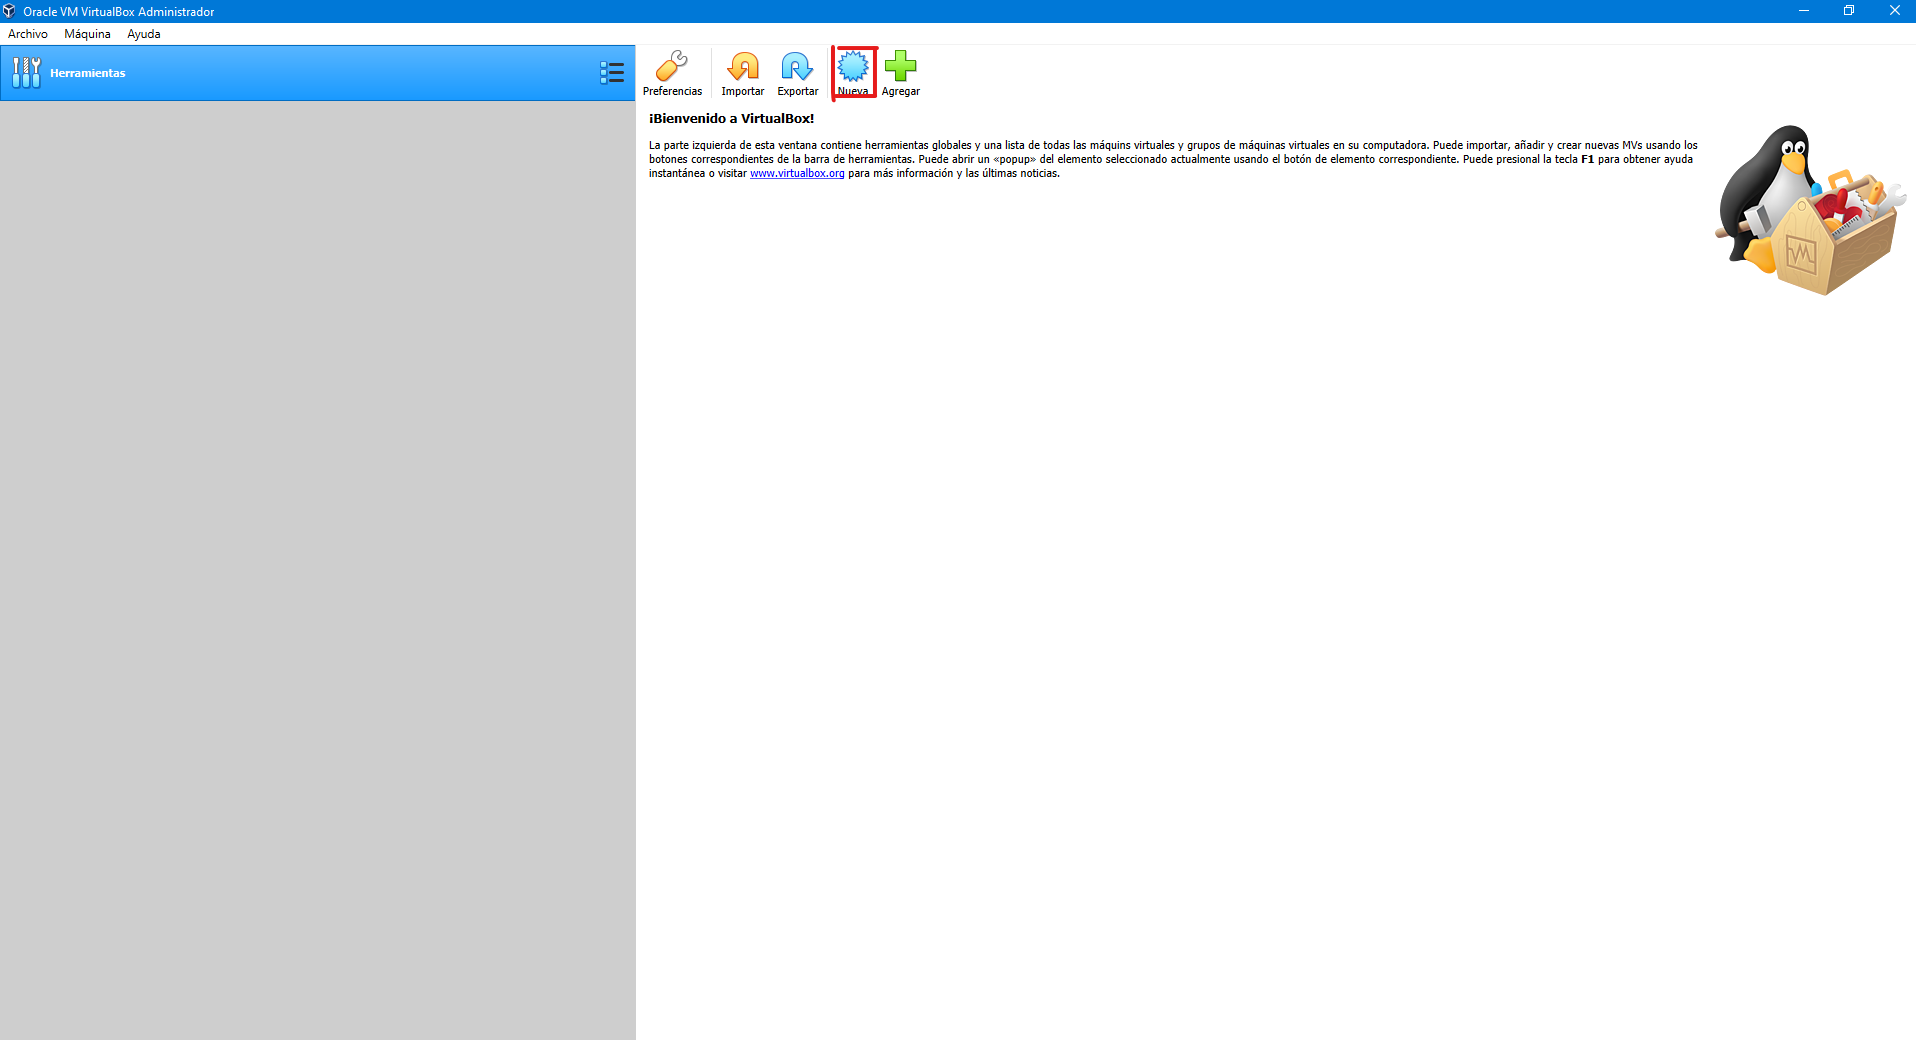
\includegraphics[width= 0.7 \textwidth]{Media/VB1.png}
    \end{figure}
    
\subsection{Configuración Inicial}
\noindent
A continuación daremos un nombre a nuestra Máquina Virtual, seleccionaremos la carpeta donde la vamos a crear y escogeremos el tipo de máquina (en nuestro caso Linux) y su versión (la distribución principal a la que corresponda, en nuestro caso ARCH Linux, pues instalaremos Manjaro).
    \begin{figure}[H]
        \centering
        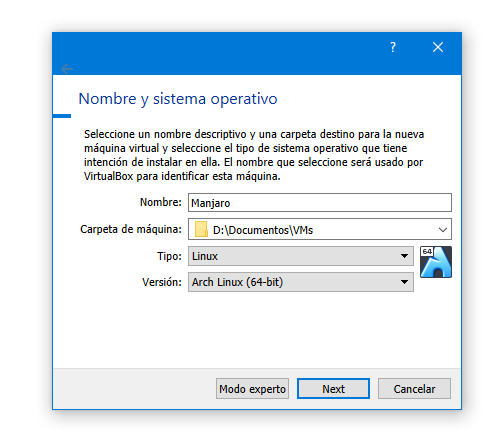
\includegraphics[width= 0.7 \textwidth]{Media/VB2.png}
    \end{figure}
\newline \noindent Pulsamos sobre el botón \textit{'Siguiente'}.

\subsection{Tamaño de la memoria}
\noindent
Ahora seleccionaremos el tamaño de memoria RAM que queremos asignar a nuestra Máquina Virtual. Por defecto nos pone 1024MB, yo os recomiendo subir al menos a 2048MB si vuestro PC tiene 8GB o más de memoria RAM instalada. Tened en cuenta que debéis dejar memoria suficiente para que Windows administre el resto del sistema.
    \begin{figure}[H]
        \centering
        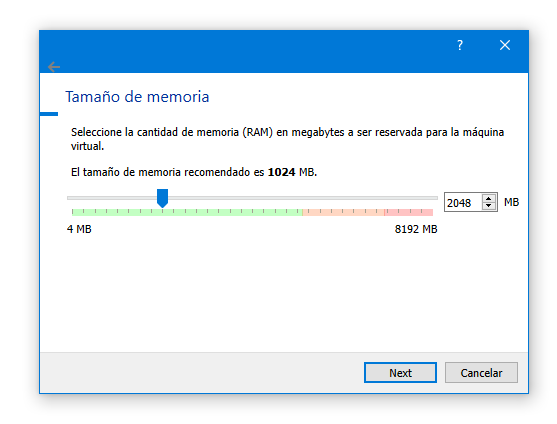
\includegraphics[width= 0.7 \textwidth]{Media/VB3.png}
    \end{figure}
\newline \noindent Pulsamos sobre el botón \textit{'Siguiente'}.

\subsection{Creación de un Disco Duro Virtual}
\noindent
\subsubsection{Creación}
Nuestra máquina necesita estar alojada en algún espacio físico, para ello crearemos una pequeña partición en nuestro disco (un Disco Duro Virtual).
\begin{figure}[H]
        \centering
        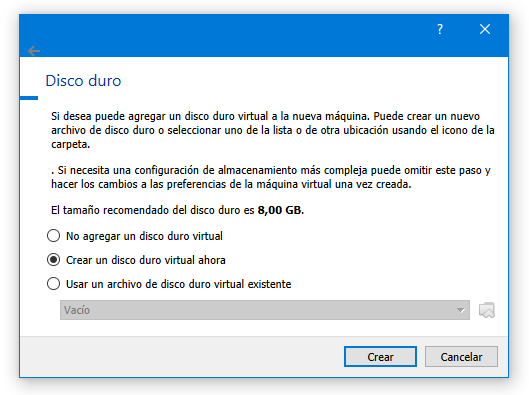
\includegraphics[width= 0.7 \textwidth]{Media/VB4.png}
    \end{figure}
\newline \noindent Pulsamos sobre el botón \textit{'Crear'}.

\subsubsection{Tipo de Disco Duro}
\noindent
VirtualBox nos ofrece 3 opciones, de las cuales, tanto la primera (\textit{VirtualBox Disk Image}, como la segunda (\textit{Virtual Hard Disk}, son recomendables. Lo dejamos a vuestra elección.
\begin{figure}[H]
        \centering
        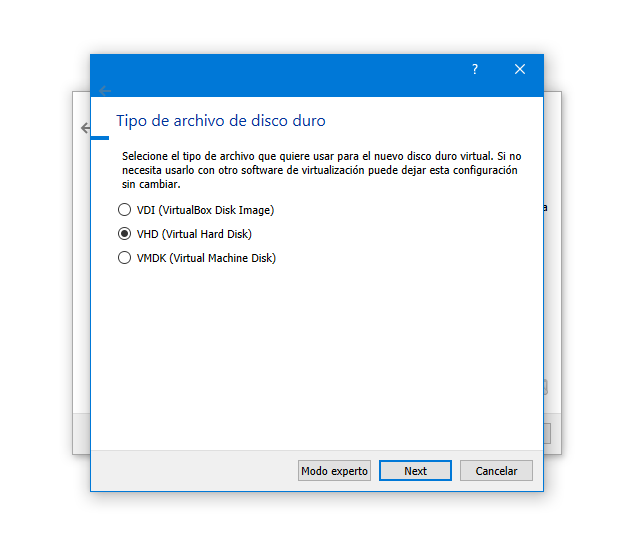
\includegraphics[width= 0.7 \textwidth]{Media/VB5.png}
    \end{figure}
\newline \noindent Pulsamos sobre el botón \textit{'Siguiente'}.

\subsubsection{Tipo de Almacenamiento}
\noindent
En este caso, VirtualBox nos ofrece 2 opciones:
\begin{enumerate}
    \item Reservado dinámicamente: esto irá ocupando espacio en nuestro disco según la Máquina Virtual necesite, hasta el máximo que le asignaremos a continuación.
    \item Tamaño fijo: reservará directamente todo el espacio que le digamos a continuación, tanto si la Máquina Virtual lo está usando, como si no.
\end{enumerate}
\begin{figure}[H]
        \centering
        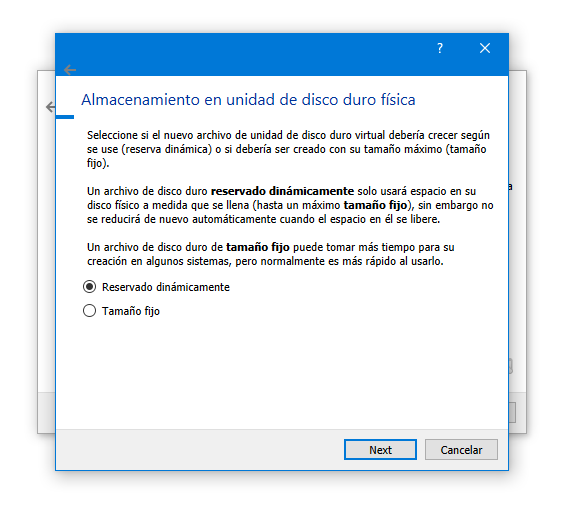
\includegraphics[width= 0.7 \textwidth]{Media/VB6.png}
    \end{figure}
\newline \noindent Pulsamos sobre el botón \textit{'Siguiente'}.

\subsubsection{Ubicación y tamaño}
\noindent
En este apartado podremos seleccionar la ubicación en la que se creará el Disco Duro Virtual. Además, VirtualBox nos recomienda el tamaño mínimo para que la Máquina Virtual funcione, podemos asignar más si así lo queremos.
\begin{figure}[H]
        \centering
        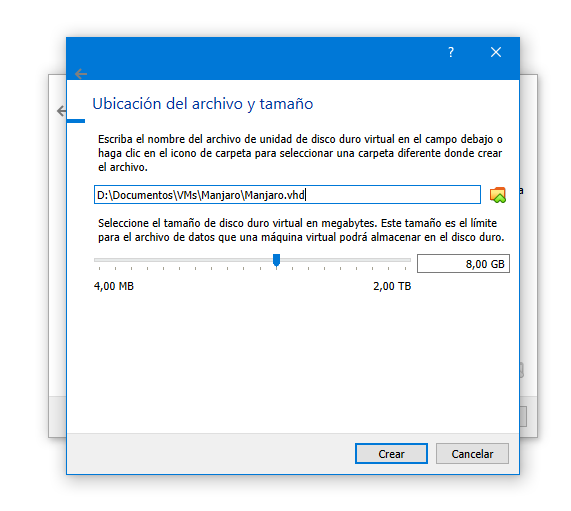
\includegraphics[width= 0.7 \textwidth]{Media/VB7.png}
    \end{figure}
\newline \noindent Pulsamos sobre el botón \textit{'Crear'}.

\subsection{Selección de la ISO}
\noindent
Ahora vamos a decirle a VirtualBox de dónde tiene que leer la ISO para instalar la Máquina Virtual.
\begin{figure}[H]
        \centering
        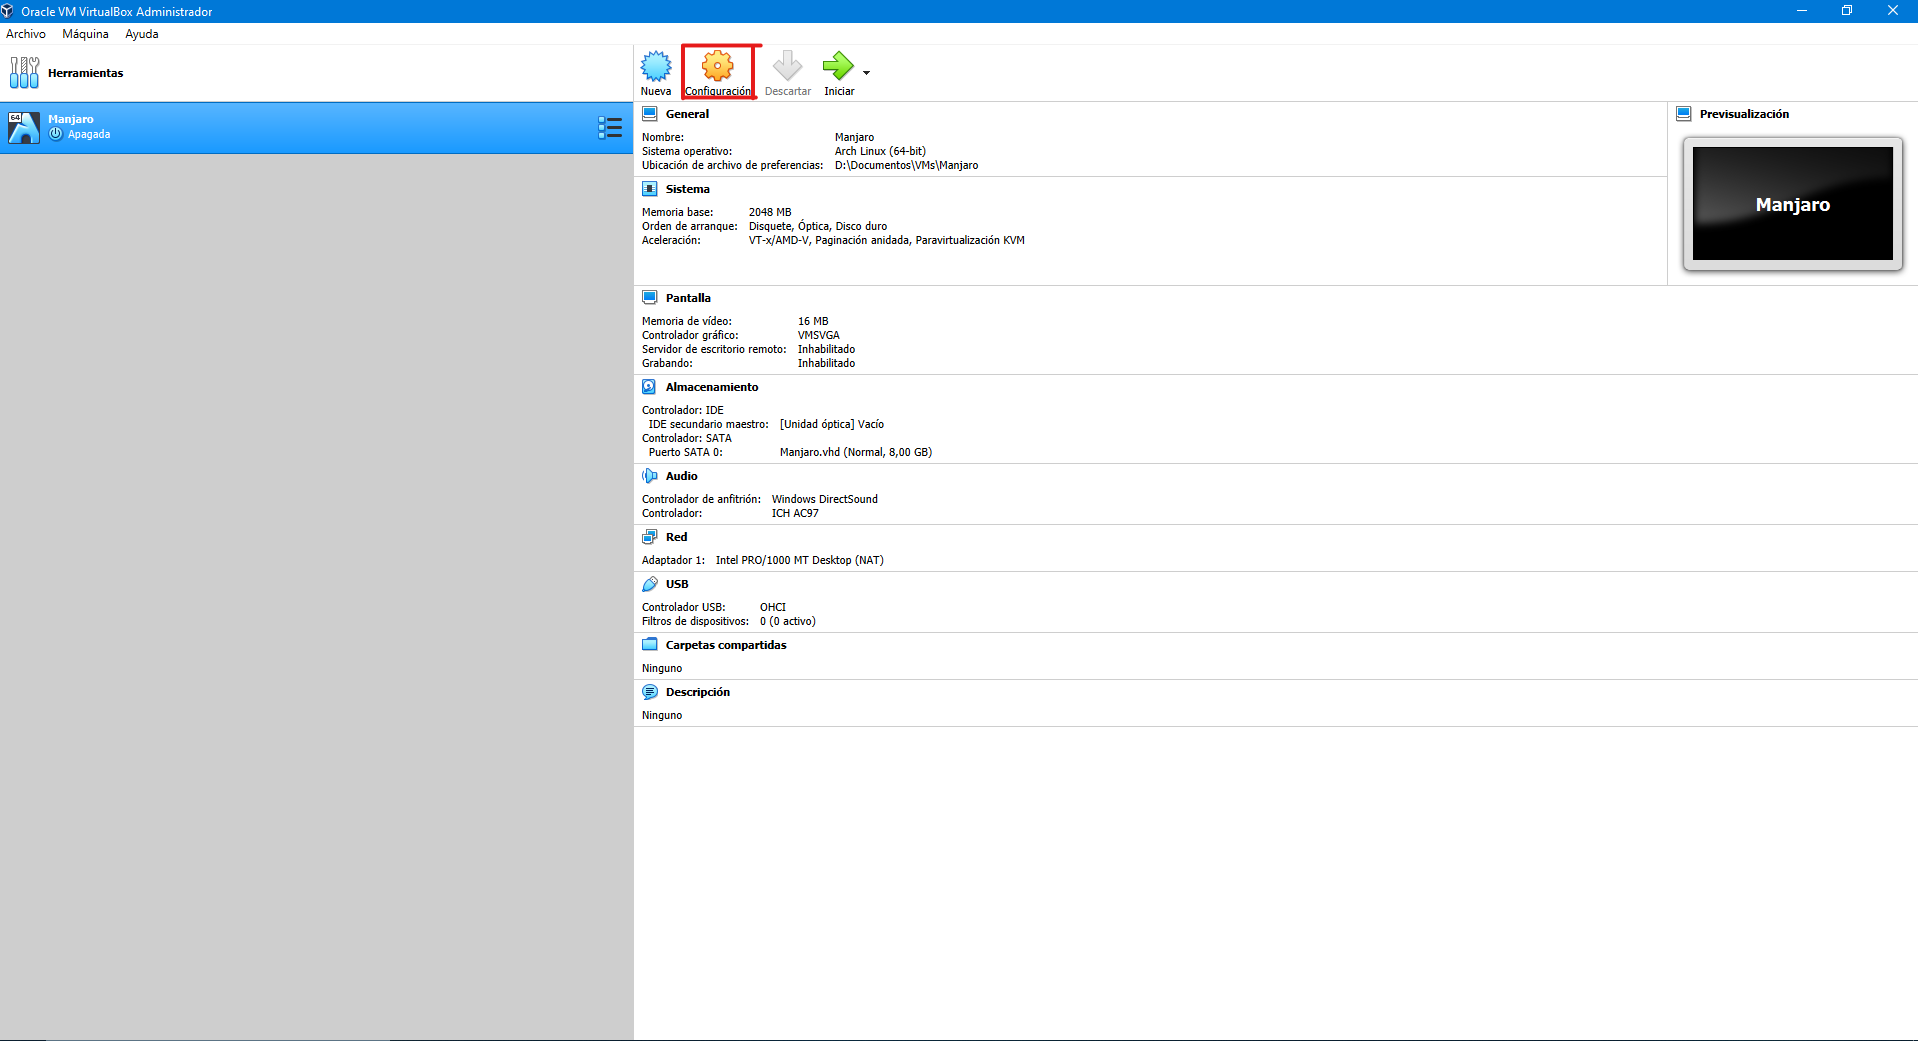
\includegraphics[width= 0.7 \textwidth]{Media/VB8.png}
    \end{figure}
\newline \noindent Pulsamos sobre el botón \textit{'Configuración'}.
\begin{figure}[H]
        \centering
        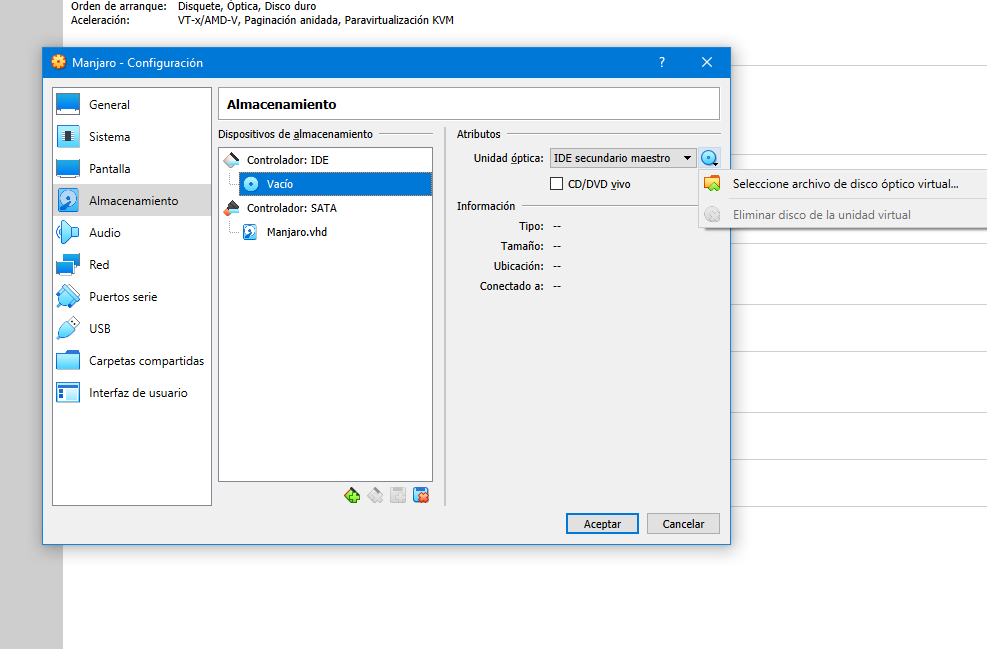
\includegraphics[width= 0.7 \textwidth]{Media/VB9.png}
    \end{figure}
\newline \noindent Vamos a la sección de \textit{'Almacenamiento'} y en el \textit{'Controlador'}, seleccionamos el archivo de disco óptico virtual (lo que sería el medio de instalación).
\begin{figure}[H]
        \centering
        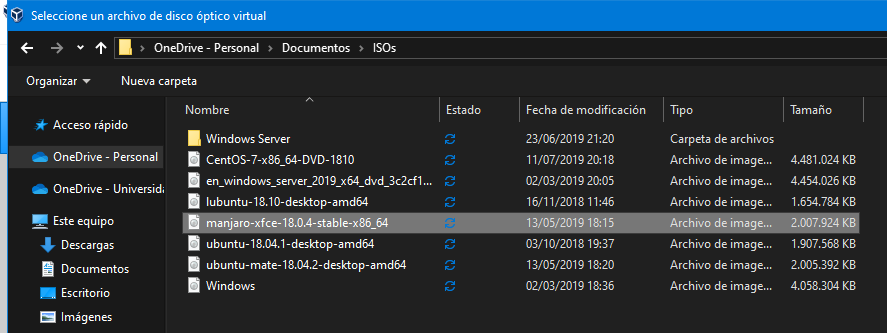
\includegraphics[width= 0.7 \textwidth]{Media/VB10.png}
    \end{figure}
\newline \noindent Buscamos la carpeta donde habíamos guardado la ISO y la seleccionamos.
\begin{figure}[H]
        \centering
        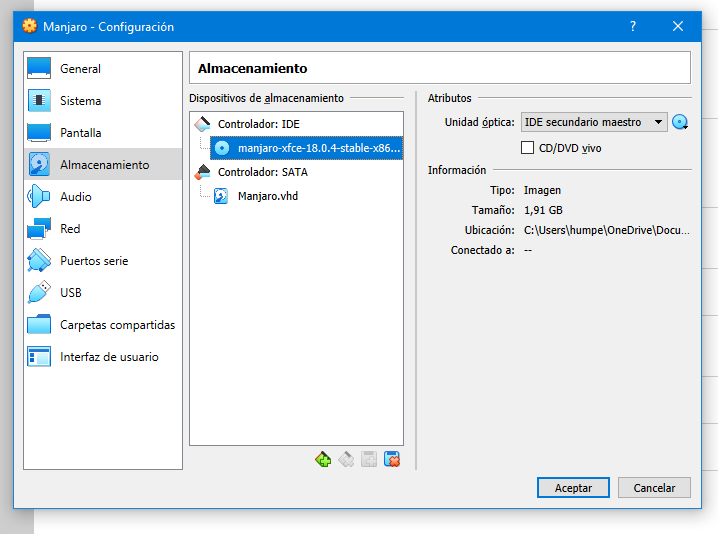
\includegraphics[width= 0.7 \textwidth]{Media/VB11.png}
    \end{figure}
\newline \noindent Pulsamos sobre el botón \textit{'Aceptar'} y listo.
\begin{figure}[H]
        \centering
        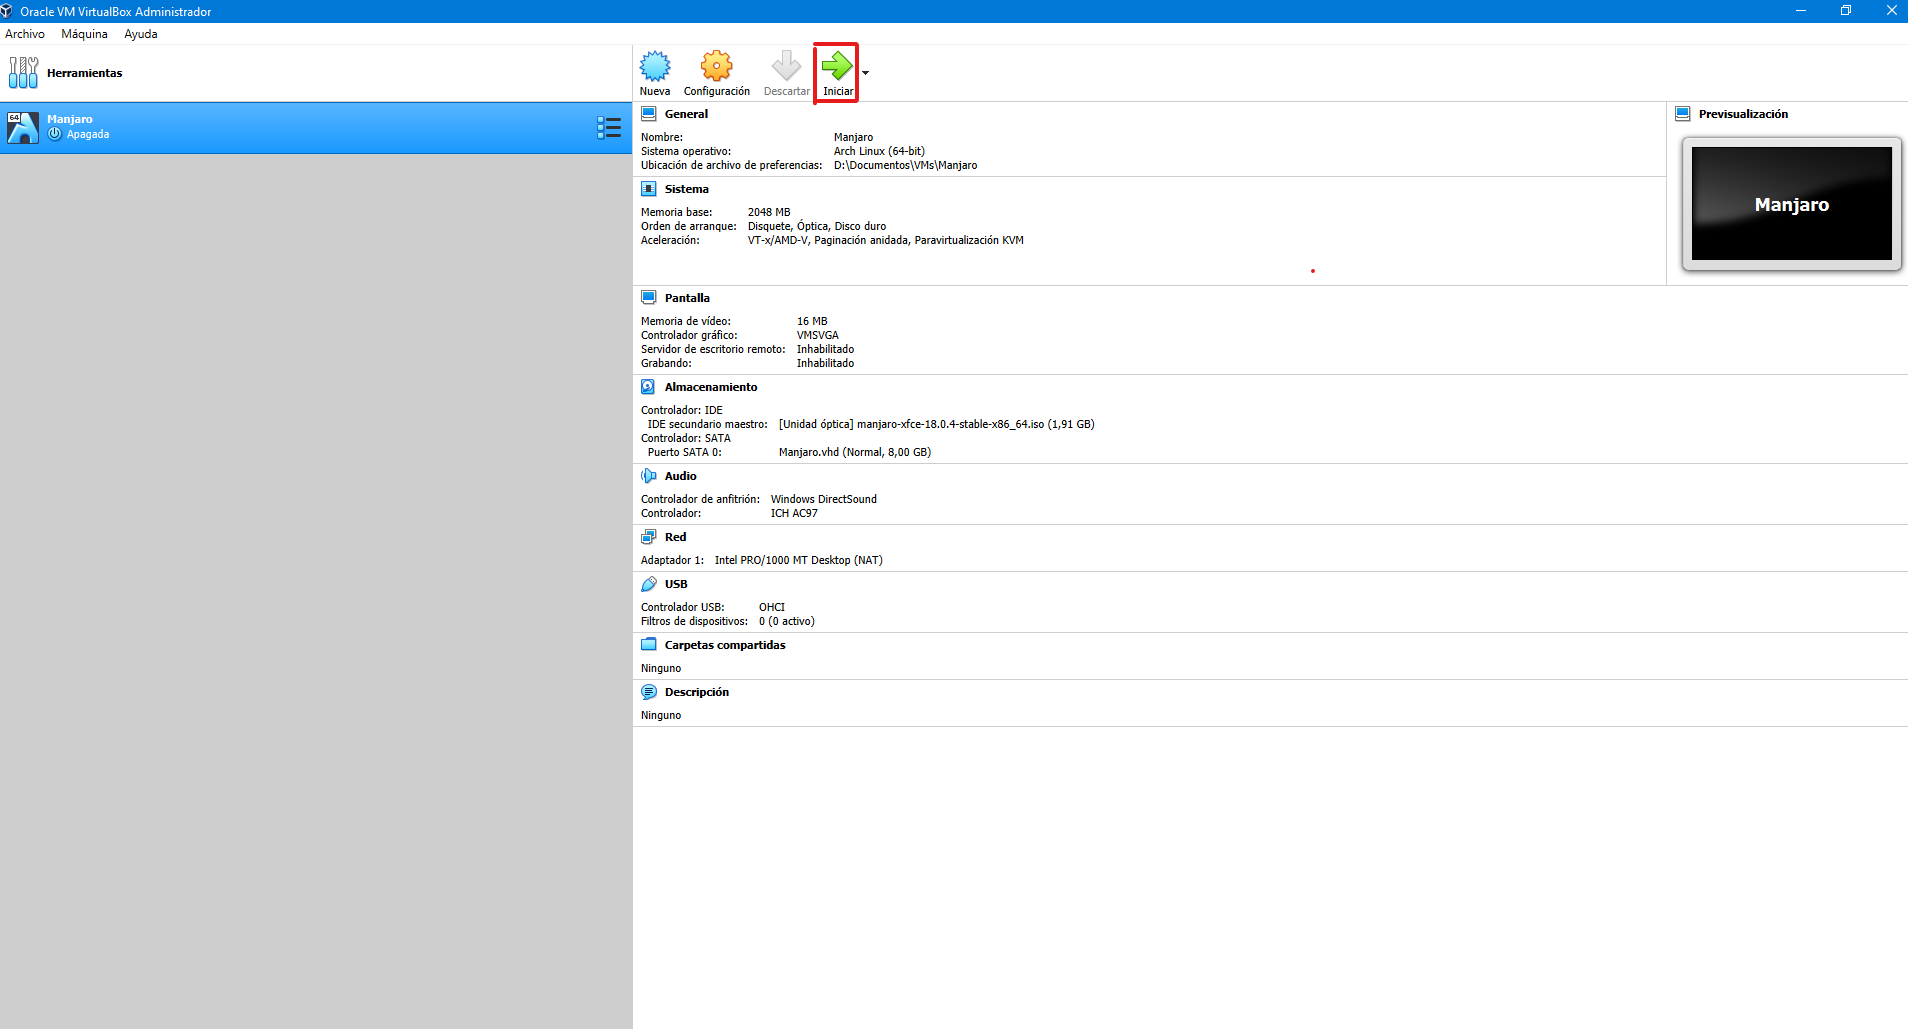
\includegraphics[width= 0.7 \textwidth]{Media/VB12.png}
    \end{figure}
\newline \noindent Ahora ya sólo tenemos que pulsar sobre el botón \textit{'Iniciar'} de la Máquina Virtual y comenzará la instalación. Para guiaros, podéis seguir la guía de instalación del apartado \textbf{\textit{2.Instalación de Linux}}, a partir del punto \textbf{\textit{2.4.Opciones de Instalación}}.
